\newpage
\section{Principio de Inducción Matemática}\label{mathematical-induction}

\subsection{Defininciones}

La Inducción Matemática es una técnica utilizada para probar declaraciones o proposiciones.
La idea es similar a la de hacer caer varias piezas de dominó.
Si cada pieza está lo suficientemente cerca de la anterior y hacemos caer la primera, entonces todas las piezas eventualmente van a caer.
Cuando queremos probar una proposición sobre números naturales, la idea es la misma.
En la Figura~\ref{fig:figure} podemos ver una representación gráfica de esta analogía.

\begin{figure}[htb]
    \centering
    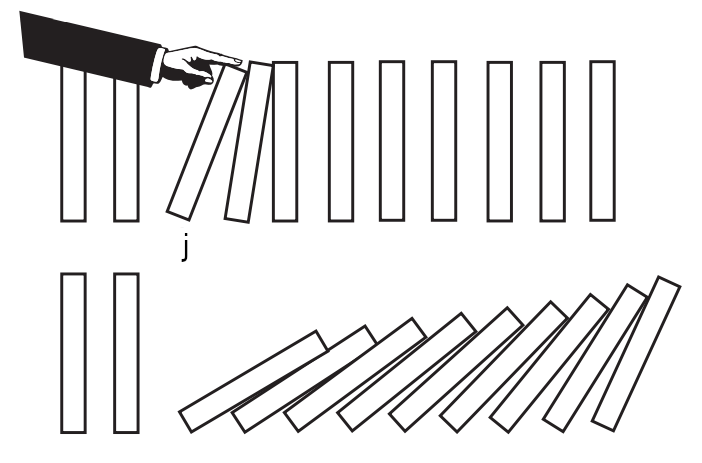
\includegraphics[width=8cm]{images/dominoes-fall}
    \caption{Fichas de dominó cayendo.}
    \label{fig:figure}
\end{figure}

\begin{section-theorem.tcb}{Principio de Inducción Matemática}{}
    Para algún entero fijo $j$ y para cada entero $n \geq j$, sea $S(n)$ una declaración\footnote{También podemos decir Proposición o Afirmación} que involucre a $n$. Si
    \begin{itemize}
        \item $S(j)$ es cierto, y
        \item para cada entero $k \geq j$, $S(k) \rightarrow S(k + 1)$,
    \end{itemize}
    entonces para todo $n \geq j$, la declaración $S(n)$ es cierta.
\end{section-theorem.tcb}

Una manera de estructurar la solución de un problema que resolvemos por inducción matemática es la siguiente.
\begin{enumerate}
    \item \textbf{Base de inducción (o caso base)}\\
    Probar que $S(1)$ es cierta (generalmente $j$ será 1).

    \item \textbf{Hipótesis de inducción}\\
    Suponer que para un entero fijo $k \geq 1$, la declaración $S(k)$ es cierta.

    \item \textbf{Paso de inducción}\\
    Probar que como $S(k)$ es cierta, entonces $S(k + 1)$ también será cierta.
\end{enumerate}

\begin{section-example.tcb}
    Sea $m$ entero positivo, probar que para $m \geq 3$, se cumple \[m^m > 2m!.\]
\end{section-example.tcb}

\begin{solution}
    Tomemos por $S(m)$ la afirmación $m^m > 2m!$.

    \textbf{Base de inducción}\\
    Tomando $m = 3$, vemos que $3^3 > 2\cdot3!$, por lo tanto $S(3)$ es cierta.

    \textbf{Hipótesis de inducción}\\
    Supongamos que $S(k)$ es cierta para algún entero fijo $k\geq 3$.

    \textbf{Paso de inducción}\\
    Probaremos, entonces que si $S(k)$ es cierta, $S(k + 1)$ también será cierta.
    Esto es
    \[(k + 1)^{k + 1} > 2(k + 1)!\]
    Notemos que
    \begin{gather*}
    (k + 1)^{k}\cdot(k + 1)^1 > 2(k + 1)\cdot k!\\
    (k + 1)^k > 2k!
    \end{gather*}
    Ahora bien, es claro que $k + 1 > k$, por lo tanto $(k + 1)^k > k^k$.
    Así por la hipótesis de inducción tendremos lo siguiente.
    \[(k + 1)^k > k^k > 2k!\]
    Es decir, $S(m)$ es cierta para toda $m\geq 3$.
    Luego, la prueba está hecha.
\end{solution}

\begin{section-theorem.tcb}{Binomio de Newton}{}
    Para $a$ y $b$ números reales y $n$ un número entero, se cumplirá que
    \[(a + b)^n = \binom{n}{0}a^n + \binom{n}{1}a^{n - 1}b + \cdots + \binom{n}{i}a^{n - i}b^i + \cdots + \binom{n}{n}b^n.\]
\end{section-theorem.tcb}

Podemos utilizar la notación de sumatoria y quedaría como:
\[(a + b)^n = \sum\limits_{i = 0}^{n} \binom{n}{i}a^{n - i}b^i.\]

\begin{proof}
    La demostración la haremos por inducción sobre $n$.
    Si $n = 0$, entonces $(a + b)^0 = 1$ y $\binom{0}{0}a^0 b^0 = 1$.
    Supongamos que para un entero fijo $k \geq 0$ la declaración es cierta, es decir
    \[
        (a + b)^k = \sum\limits_{i = 0}^{k} \binom{k}{i}a^{k - i}b^i
    \]
    es válida, entonces
    \begin{align*}
        (a + b)^{k + 1} &= (a + b)(a + b)^k\\
        &= (a + b) \sum\limits_{i = 0}^{k} \binom{k}{i}a^{k - i}b^i\\
        &= a\sum\limits_{i = 0}^{k} \binom{k}{i}a^{k - i}b^i + b\sum\limits_{i = 0}^{k} \binom{k}{i}a^{k - i}b^i\\
        &= a\left[\binom{k}{0}a^{k} + \sum\limits_{i = 1}^{k} \binom{k}{i}a^{k - i}b^i\right] + b\left[\sum\limits_{i = 0}^{k - 1} \binom{k}{i}a^{k - i}b^i + \binom{k}{k}b^k\right]\\
        &= \binom{k}{0}a^{k + 1} + \sum\limits_{i = 1}^{k} \binom{k}{i}a^{k + 1 - i}b^i+ \sum\limits_{i = 0}^{k - 1} \binom{k}{i}a^{k - i}b^{i + 1} + \binom{k}{k}b^{k + 1} \\
        &= \binom{k}{0}a^{k + 1} + \sum\limits_{i = 1}^{k} \binom{k}{i}a^{k + 1 - i}b^i+ \sum\limits_{i = 1}^{k} \binom{k}{i - 1}a^{k + 1 - i}b^{i} + \binom{k}{k}b^{k + 1} \\
        &= \binom{k + 1}{0}a^{k + 1} + \sum\limits_{i = 1}^{k} \left[ \binom{k}{i} + \binom{k}{i - 1}\right] a^{k + 1 - i}b^i + \binom{k + 1}{k + 1}b^{k + 1} \\
        &= \binom{k + 1}{0}a^{k + 1} + \sum\limits_{i = 1}^{k} \binom{k + 1}{i} a^{k + 1 - i}b^i + \binom{k + 1}{k + 1}b^{k + 1} \\
        (a + b)^{k + 1} &= \boxed{\sum\limits_{i = 0}^{k + 1} \binom{k + 1}{i} a^{k + 1 - i}b^i} \qedhere
    \end{align*}
\end{proof}



\subsection{Agregados culturales y preguntas}

    \begin{enumerate}
        \item { \textbf{Otra analogía.}
        Considera una pila de sobres, tan alta como querás.
        Supongamos que cada sobre tiene el mismo mensaje en su interior ''\textit{Abre el siguiente sobre de la pila, y sigue las instrucciones escrito en él}''.
        Si alguien abre el primero (el de arriba), lee el mensaje y sigue las instrucciones, entonces la persona se ve obligada a abrir el segundo sobre.
        Y si la persona decide seguir cada instrucción, entonces esta persona abrirá todos los sobres de la pila.
        Es decir, esto es el principio de Inducción Matemática aplicado a una pila de sobres.}

        \item La \textbf{Inducción fuerte} es una variante de la Inducción Matemática "normal". Esta surge cuando para probar $S(k + 1)$ es necesario considerar más de una declaración previa como cierta $S(i), S(i + 1), \cdots, S(k)$. Muchas veces no hace falta usar todas las declaraciones anteriores, pero sí al menos un par de ellas (dependerá del problema).
    \end{enumerate}


\subsection{Ejercicios y Problemas}

    Sección de ejercicios y problemas para el autoestudio.

    \begin{section-problem}
        Probar que $\forall n \in \ZP$, se cumple que $1^2 + 2^2 + \dots + n^2 = \dfrac{n(n+1)(2n+1)}{6}$.
    \end{section-problem}

    \begin{section-problem}
        Probar que $\forall n\in \ZP$, $4007^n - 1$ es divisible por 2003.
    \end{section-problem}

    \begin{section-problem}
        Probar que $\forall n \in \ZP$, el número $A_n = 3^n - 2n^2 - 1$ es múltiplo de $8$.
        Además que si $3\nmid n$, entonces $A_n$ es múltiplo de 24.
    \end{section-problem}

    \begin{section-problem}
        Sea $\{a_n\}$ una secuencia tal que $a_1 = 5$, $a_2 = 13$ y $a_{n+2}=5a_{n+1}-6a_n\text{,}\ \forall n \in \N$.
        Probar que $a_n = 2^n+3^n \text{,}\ \forall n \in \N$.
    \end{section-problem}

    \begin{section-problem}
        Sea $q \in \R$, con $q \neq 1$ y $n \in \Z^{\geq 0}$.
        Probar que
        \[(1 + q)(1 + q^2)(1 + q^4)\cdots(1 + q^{2^n}) = \frac{1 - q^{2^{n + 1}} }{1 - q}.\]
    \end{section-problem}

    \begin{section-problem}
        Demostrar que $\forall a, b\in \R^+$ y $n \in \N$ se cumple que $2^{n - 1}(a^n + b^n) \geq (a + b)^n.$
    \end{section-problem}

    \begin{section-problem}
        Probar $\forall n \in \N$, que se cumple $F_1 + F_3 + \cdots + F_{2n - 1} = F_{2n}.$ ($F_n$ es la sucesión de Fibonacci.)
    \end{section-problem}

    \begin{section-problem}
        Probar $\forall n \in \N^{\geq 2}$, que se cumple $F_{2n} = F_{n + 1}^2 - F_{n - 1}^2.$
    \end{section-problem}